\documentclass[a4paper]{scrreprt}
	
\usepackage[T1]{fontenc}
\usepackage[ngerman]{babel}     % deutsche Silbentrennung
\usepackage[utf8x]{inputenc}    % wegen deutschen Umlauten & UTF-8
\usepackage{lmodern}		% Schönere Schriftart
\usepackage{graphicx}           % Grafikpaket laden
\usepackage{amsmath,amssymb}    % Mathe
\usepackage{tikz}               % Zeichungen
\usepackage{hyperref}		% Links
\hypersetup{			% Link-Formatierung entfernen & pdf-Inforamtionen setzten
	pdfauthor={Maximilian Awiszus, Holger Ebhart, Lidia Grigoriev, Paul Jungeblut, Philipp Kern  und Matthias Schimek},
	pdftitle={Visualizing Trends - Was verrät uns Twitter?},
	colorlinks,
	citecolor=black,
	filecolor=black,
	linkcolor=black,
	urlcolor=black
}
\usepackage{microtype}		% font expansion

\title{Visualizing Trends\\Was verrät uns Twitter?}
\subtitle{Pflichtenheft}
\author{Maximilian Awiszus\and Holger Ebhart\and Lidia Grigoriev\and Paul Jungeblut\and Philipp Kern\and Matthias Schimek}

\begin{document}
	\maketitle
	\tableofcontents
	\chapter{Einleitung}
		% vollständige Beschreibung der Aufgabenstellung.

	\chapter{Zielbestimmungen}
		% Beschreibt die Funktionalität der zu entwickelnden Systemkomponente. 
% o Musskriterien: Mindestanforderungen, gehen aus Aufgabenstellung hervor. 
% o Wunschkriterien: Von den Gruppen selbst definierte, zusätzliche Funktionalität. 
% o Abgrenzungskriterien: Was gehört nicht zum Funktionsumfang? (vgl. auch Produkteinsatz) 

\section{Musskriterien}
\begin{itemize}
	\item Es soll ein Programm entwickelt werden, dass Twitterdaten (mittels Streaming- und Search-API) nach verifizierten Nutzern durchsucht und diese speichert.
	\item Zu Tweets von verifizierten Accounts sollen Retweets geografisch gruppiert und gezählt werden.
	\item Dazu soll einzelnen Accounts eine geografische Position und eine thematische Kategorie zugeordnet werden.
	\item Es sollen interaktiv Anfragen an das System gestellt werden können: Anfragen bestehen zum Beispiel aus einer Kategorie und einem Land. Damit soll die weltweite geografische Ausbreitung von Tweets mit diesen Eigenschaften grafisch dargestellt werden (siehe \cref{sec:Produktfunktionen}).
	\item Die Interaktion mit dem System soll über eine intuitiv bedienbare grafische Benutzeroberfläche geschehen. Diese soll neben den Auswahlhilfen eine Weltkarte sowie weitere Statistiken zeigen.
	\item Über die Benutzeroberfläche sollen Accounts manuell kategorisiert und lokalisiert werden können.
\end{itemize}

\section{Wunschkriterien}
Folgende Auflistung zeigt die Wunschkriterien in absteigender Priorität.
\begin{enumerate}
	\item Es soll möglich sein, nicht verifizierte Benutzer einzugeben, sodass die Ausbreitung ihrer Tweets analysiert werden kann.
	\item Visualisierung von Datenströmen auf der Karte.
	\item Eine Visualisierung der Analyseergebnisse mit Schwerpunkt auf der zeitlichen Entwicklung sowie weiterer Statistiken wie der Häufigkeit bestimmter Kategorien in verschiedenen Ländern.
	\item Eine hierarchische Einteilung der Regionen in Ergänzung zur Analyse pro Land. So könnte zum Beispiel pro Kontinent  visualisiert werden.
	\item Exportfunktion für Analyseergebnisse.
\end{enumerate}

\section{Abgrenzungskriterien}
\begin{itemize}
	\item Es werden Retweets pro Account, nicht pro Tweet analysiert. Daher wird es nicht möglich sein, einzelne Tweets zu analysieren.
	\item Es handelt sich um ein Analyseprogramm, nicht um ein Lokalisierungsprogramm. Zur Lokalisierung soll ein existierender Webservice genutzt werden.
	\item Die Analyse beruht nicht auf dem Inhalt der Tweets (Hashtags, etc.) sondern ausschließlich auf der dem Account zugeordneten Kategorie und Ort.
\end{itemize}

	\chapter{Produkteinsatz}
		% Beschreibt  Einsatzgebiete,  Zielgruppe  und  Betriebsbedingungen  sowie  notwendige Hard‐ und Software.
\section{Einsatzgebiet}
Die Software wird dazu verwendet die Anzahl der Retweets einer Kategorie von Tweets in einem Land in anderen Ländern zu analysieren. Einsatzgebiete sind somit u.a.:
\begin{itemize}
	\item Statistik
	\item Marktforschung
	\item Privat
\end{itemize}
\section{Zielgruppe}
Entsprechend oben genannter Einsatzgebiete richtet sich die Anwendung an folgende Zielgruppen:
\begin{itemize}
	\item Meinungsforscher
	\item Journalisten
	\item Privatpersonen
\end{itemize}
\section{Betriebsbedingungen}
Da die Anwendung aus Server und Client besteht muss für die Betriebsbedingungen unterschieden werden.
\subsection{Client}
\begin{itemize}
				\item Bei der aus Abschnitt \ref{sec:empfohleneHardware} gegebener Hardware darf die Anzahl parallel laufender GUIs 100 Instanzen nicht überschreiten.
\end{itemize}
\subsection{Server}

	\chapter{Produktumgebung}
		% Notwendige Hard‐ und Software.
\section{Software}
   \begin{itemize}
      \item Java Runtime Environement SE 1.7 oder höher
      \item MySQL-Datenbank
      \item Betriebssystem z.B. Windows, Linux, MacOS
   \end{itemize}
\section{Hardware}
\label{sec:empfohleneHardware}
   \subsection{Server}
	Minimalanforderungen:
   \begin{itemize}
      \item Hauptspeicher 4 GB
      \item freier Festplattenspeicher 20 GB
      \item Mindestens 2 GHz Multicore-Prozessor
   \end{itemize}
   Empfohlene Hardware:
   \begin{itemize}
      \item Hauptspeicher 8 GB
      \item freier Festplattenspeicher 100 GB
      \item Mindestens 2-3 GHz Quadcore-Prozessor
   \end{itemize}
   \subsection{Client}
   	Minimalanforderungen:
   \begin{itemize}
      \item Hauptspeicher 2 GB
      \item freier Festplattenspeicher 100 MB GB
      \item Mindestens 1 GHz Prozessor
   \end{itemize}
   Empfohlene Hardware:
   \begin{itemize}
      \item Hauptspeicher mind. 4 GB
      \item freier Festplattenspeicher 200 MB
      \item Mindestens 2 GHz Multicore-Prozessor
   \end{itemize}
\section{Schnittstellen}
   \begin{itemize}
   \item Webschnittstelle (Internetzugang) mindestens 4 MB/s, empfohlen 16 MB/s
   \end{itemize}
	\chapter{Produktfunktion}
		% Detailliertere  Beschreibung  der  Funktionalität,  wiederum  gegliedert  in Grundfunktionen und optionale Funktionen. 

Die Beschreibung der Funktionalität gliedert sich in Grundfunktionen und optionale Funktionen.

\section{Grundfunktionen}

Die Grundfunktionen der Anwendung gliedern sich in verschiedene Bereiche.

%\subsection{Allgemeine Funktionalität}
%\begin{enumerate}[align=left, label={\textbf{\textbackslash F00\arabic*0\textbackslash}} ]
%	\item Start des Programms \\
%	Bei Start des Programms wird die leere Weltkarte angezeigt.
%	\begin{itemize}
%		\item Hier könnte auch Ihre Werbung stehen ...
%	\end{itemize}


%\end{enumerate}
\subsection{Auswahl der gewünschten Daten} \label{sec:Produktfunktionen}
\begin{enumerate}[ align=left, label={\textbf{\textbackslash F10\arabic*0\textbackslash}} ]
	\item \textbf{Auswahl der Kategorien} \label{PF:KategorienAuswahl}\\ 
	Die verschiedenen Kategorien werden angezeigt. Man kann durch die Auswahl navigieren und eine oder mehrere Kategorien auswählen. Hierfür kann eine Suchfunktion genutzt werden ($\rightarrow$ \ref{PF:Suchfunktion}). 
	\item \textbf{Auswahl der Ortsbeschränkung} \label{PF:OrtAuswahl} \\
	Die verschiedenen Orte werden angezeigt. Man kann durch die Auswahl navigieren und einen oder mehrere Orte auswählen. Hierfür kann eine Suchfunktion genutzt werden ($\rightarrow$ \ref{PF:Suchfunktion}). 
	\item \textbf{Manuelles Hinzufügen weiterer Accounts} \label{PF:AccountHinzufügen} \\
	Mittels der Suchfunktion ($\rightarrow$ \ref{PF:Suchfunktion}) können weitere Accounts einzeln zur Auswahl hinzugefügt werden, sofern diese in der Datenbank hinterlegt sind.
	\item \textbf{Suchfunktion innerhalb des Auswahlprozesses} \label{PF:Suchfunktion} \\
	Es kann nach Kategorien, Orten und Benutzern gesucht werden, die bereits in der Datenbank vorhanden sind. Die Funktionalität unterscheidet sich je nach der Art des gesuchten Objekts. In allen Fällen wird eine Liste mit Vorschlägen abhängig vom gerade eingegebenen Suchbegriff angezeigt. 
	\item \textbf{Aktualisierung der Anfrage} \label{PF:Absenden} \\
	Bei Änderung der Anfrageparameter werden die Daten automatisch ausgewertet und nach einer gewissen Latenzzeit angezeigt.
\end{enumerate}	
\subsection{Visualisierung der Daten}	
Für die Visualisierung der Daten bestehen folgende Funktionen.
\begin{enumerate}[ align=left, label={\textbf{\textbackslash F20\arabic*0\textbackslash}} ]	
	\item \textbf{Anzeige der grafisch aufbereiteten Daten} \label{PF:Visualisieren}\\
	Die Daten der aktuellen Anfrage werden grafisch aufbereitet in der Karte dargestellt.
	\begin{itemize}
		\item Einfärben der Karte ($\rightarrow$ \ref{PF:EinfärbenKarte}).
		\item Detaillierte Informationen bezüglich einzelner Orte ($\rightarrow$ \ref{PF:DetailsKarte}).
	%	\item Wahl des Beobachtungszeitraums ($\rightarrow$ \ref{PF:WahlZeitraum}).
	%	\item Anzeige von Veränderungen des Tweet-Retweet-Verhaltens über einen Zeitraum ($\rightarrow$ \ref{PF:Diff})
	\end{itemize}
	
	\item \textbf{Einfärben der Karte} \label{PF:EinfärbenKarte} \\
	Die Länder/Regionen werden auf der Karte bezüglich der Tweet-Retweet-Intensität unterschiedlich eingefärbt. Hierbei handelt es sich um relative Daten, um Bevölkerungsunterschiede auszugleichen.
	\item \textbf{Detaillierte Informationen bezüglich einzelner Orte} \label{PF:DetailsKarte} \\
	Beim Bewegen des Mauszeigers über einen Ort werden detaillierte Informationen wie Anzahl der Retweets über die Tweet-Retweet-Beziehung der aktuellen Anfrage an diesem Ort angezeigt. Diese Option kann deaktiviert werden.
	
	
	\item \textbf{Anzeige mittels Datenblatt} \label{PF:AnzeigeDatenblatt} \\
	Die relevanten Daten der Anfrage werden in Tabellenform dargestellt. Zu einem Ort-Kategorie-Paar können die zugehörigen Accounts aufgelistet werden.
	

\end{enumerate}

\subsection{Navigation auf der Weltkarte}
\begin{enumerate}[ align=left, label={\textbf{\textbackslash F30\arabic*0\textbackslash}} ]
	\item \textbf{Navigation auf der Karte} \label{PF:Navigation} \\
	Es ist möglich die Karte zu verschieben.
	\item \textbf{Zoomen} \label{PF:Zoomen} \\
	Die Ansicht auf die Karte kann, innherhalb gewisser Grenzen, vergrößert und verkleinert werden.
\end{enumerate}	
\subsection{Manuelle Bearbeitung der Datenbank}
Durch den Benutzer können einige Änderungen der in der Datenbank  gespeicherten Daten vorgenommen werden. Diese Funktionen müssen gegebenenfalls eingeschränkt werden, sollte die Anwendung öffentlich verwendet werden.
\begin{enumerate}[ align=left, label={\textbf{\textbackslash F40\arabic*0\textbackslash}}]
	\item \textbf{Kategorie eines Accounts ändern}  \label{PF:KategorieAendern} \\
	Die Kategorie eines gespeicherten Accounts kann in eine schon in der Datenbank vorhandene Kategorie geändert werden.
	\item \textbf{Ort eines Accounts ändern} \label{PF:OrtAendern}\\
	Der Ort eines Account kann in einen schon in der Datenbank vorhandenen Ort geändert werden.
	\item \textbf{Account hinzufügen} \label{PF:AccountHinzu} \\
	Es kann ein Twitter-Account, sofern dieser existiert, zu der Liste der mitgelesenen Twitter-Accounts hinzugefügt werden, auch wenn dieser nicht verifiziert ist.
\end{enumerate}

\section{Optionale Funktionalität}
Die optionalen Funktionen sind nach absteigender Priorität aufgelistet.
\begin{enumerate}[ align=left, label={\textbf{\textbackslash F50\arabic*0\textbackslash}}]
	\item \textbf{Anzeigen von Veränderungen  zwischen zwei Zeitpunkten} \label{PF:Diff} \\
	Die Unterschiede in der Tweet-Retweet-Beziehung können zwischen zwei, innerhalb gewisser Grenzen, wählbaren Zeitpunkten grafisch dargestellt werden.
	\item \textbf{Wahl des Beobachtungszeitraums} \label{PF:WahlZeitraum} \\
	Der Zeitraum, für welchen die Tweet-Retweet-Beziehung dargestellt werden soll, kann innerhalb gewisser Grenzen und mit diskreten Zeitpunkten ausgewählt werden.
	\item \textbf{Allgemeine Suchfunktion} \label{PF:AllgSuche} \\
	Es wird eine allgemeine Suchfunktion angeboten. Hier kann nach beliebigen Begriffen gesucht werden. Die  Daten, welche zum jeweiligen Begriff in der Datenbank verfügbar sind, werden angezeigt.
	\item  \textbf{Sicherung von Ergebnissen} \label{PF:Sicherung} \\
	Die zu einer Anfrage erstellten Datenblätter und Kartenanzeigen können in geeignete Dateiformate exportiert und somit dauerhaft gespeichert werden.
	\item \textbf{Feingliederung der Auswahlmöglichkeiten} \\
	Es ist innerhalb einer größeren Anfrage möglich, einzelne Kategorien auf eine Teilmenge der insgesamt ausgewählten Orte zu beschränken. Man kann somit beispielsweise die Anfrage nach der Kategorie \emph{Musiker} auf den Ort \emph{Irland} einschränken und  derselben Anfrage noch die Kategorie \emph{Politiker} eingeschränkt auf den Ort \emph{Deutschland} hinzufügen.
	\item \textbf{Verknüpfung mit Twitteraccount} \label{PF:Verknuepfung} \\
	Ein Account in der Datenbank wird mit seinem Twitterprofil verknüpft. Wird der Account beispielsweise über die allgemeine Suchfunktion ($\rightarrow$ \ref{PF:AllgSuche}) gesucht und aufgerufen, werden Informationen aus der Timeline des Accounts angezeigt. 
	\item \textbf{Weitere Informationen zu Kategorien und Orten} \label{PF:WeiterInfos} \\
	Wird ein Ort oder eine Kategorie über die Suchfunktion ($\rightarrow$ \ref{PF:AllgSuche}) gesucht und aufgerufen, werden zusätzliche Informationen, die beispielsweise von wikipedia.org stammen, angezeigt.
	
	\item \textbf{Weitere Statistiken} \label{PF:Statistiken} \\
	Es werden noch weitere Statistikfunktionen und Anzeigeoptionen angeboten.
\end{enumerate}

	\chapter{Produktdaten}
		% Anfallende Daten außerhalb des Quellcodes.
\begin{itemize}
\section{GUI}
	\item[/PD1010/]Kartendaten der Länder
	\item[/PD1020/]Vom Benutzer hinzugefügte Accounts
	\item[/PD1030/]Namen aller Kategorien
	
\section{Server-Datenbank}
	\item[/PD2010/]zertifizierte Twitter-Accounts	
	\item[/PD2020/]Anzahl der Retweets pro Twitter-Account, getrennt nach Zeit und Ort
	\item[/PD2030/]Alle Twitter-Accounts zuweisbaren Kategorien
	\item[/PD2040/]Alle Orte
	\item[/PD2050/]Kategorie der zertifizierten Twitter-Accounts
	\item[/PD2060/]Lokalität der zerfifizierten Twitter-Accounts

\section{Server-Crawler}
	\item[/PD3010/]Zugangsdaten zu Twitter
\end{itemize}% Anfallende Daten außerhalb des Quellcodes.

	\chapter{Systemmodell}
		% Grobe  Architekturbeschreibung  durch  Bausteine/Komponenten  (Kein  detailliertes Klassendiagramm).

Das Projekt soll aus drei separaten Programmen bestehen. Es soll dabei keine Kommunikation untereinander stattfinden. Stattdessen greifen alle auf eine gemeinsame Datenbank zu. Eine Darstellung der drei Komponenten ist in Abbildung~\ref{c:systemmodell} zu finden.

\begin{figure}[h]
	\centering
	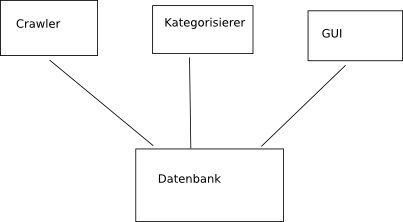
\includegraphics{img/systemmodell.png}
	\caption{Das Systemmodell}
	\label{c:systemmodell}
\end{figure}

\begin{description}
	\item[Crawler] Aufgabe des Crawlers ist es Mithilfe der Twitter-Stream- und Search-API die Twitterdaten zu sammeln. Es sollen verifizierte Benutzer und Retweets von Tweets dieser Nutzer gefunden werden. Diese Daten sollen noch im Crawler lokalisiert werden, bevor sie in der Datenbank abgespeichert werden.
	\item[Kategorisierer] Um den Crawler so leichtgewichtig wie möglich zu halten, werden die gefunden Accounts von einer weiteren Anwendung, dem Kategorisierer kategorisiert. Unabhängig vom Crawler sucht er in der Datenbank nach Accounts, denen noch keine Kategorie zugeordnet wurde. Anhand der Daten aus der DMOZ-Datenbank sollen diese Accounts dann hierarchisch kategorisiert werden. Dabei können einem Nutzer mehrere Kategorien zugeordnet werden. Der Kategorisierer arbeitet also auf den vom Crawler gefunden Daten und vervollständigt diese.
	\item[GUI] Die GUI greift lesend auf die Datenbank zu und visualisiert die Daten anhand vom Nutzer gegebener Eingaben. Sie baut somit auf Crawler und Kategorisierer auf, welche jedoch unabhängig von der GUI sind. Es ist möglich über die GUI weitere Twitteraccounts (auch nicht verifizierte) in die Datenbank aufzunehmen. Dies ist die einzige Art der Kommunikation von der GUI zur Datenbank und darüber auch zum Crawler und Kategorisierer.
\end{description}



	\chapter{Produktleistungen}
		% Wenn vorhanden, Anforderungen an Laufzeitverhalten oder Speicherplatz.
\section{Speicher}
\subsection{Server}
Durch das Sammeln von Daten mit Crawlern fällt in den ersten Wochen eine beträchtliche Menge an Daten an. Mit der Zeit, wenn ein Großteil der verifizierten Accounts gelistet ist, steigt das Volumen der Datenbank nicht mehr so stark an. Es ist dann von einer \textbf{linearen Steigerung} des Datenaufkommens auszugehen. 
Dadurch, dass der Twitterstream in Realzeit mitgelesen wird kann es zu  kurzzeitigen Peeks kommen, in denen der benötigte Hauptspeicherplatz steigt (z.B. bei hoher Anzahl an Tweets von verifizierten Accounts). Im Normalbetrieb kann allerdings von einer \textbf{stets gleich hohen Auslastung} des Hauptspeichers ausgegangen werden.
\subsection{Client}
Für die Benutzerschnittstelle (GUI) wird \textbf{kaum Festplattenspeicher} benötigt, da nur Einstellungen und benutzerdefinierte Daten lokal gespeichert werden. Die restlichen Daten werden in einer zentralen Datenbank bereitgehalten und bei Bedarf abgerufen.
Um eine flüssige Kartendarstellung zu gewährleisten wird genügend Hauptspeicherplatz benötigt (siehe \ref{subsec:hardwareClient}).
\section{Laufzeit}
\subsection{Server}
Da durch den Crawler Daten von Twitter in Realzeit gesammelt werden, können sich Beschränkungen aufgrund von Rate- und Connecting-Limits der Twitter Schnittstellen ergeben. Das Erreichen dieser Limits soll so gut wie möglich verhindert werden, allerdings können sich Verzögerungen ergeben. Es kann auch vorkommen, dass es dem Crawler für eine bestimmte Zeit nicht mehr möglich ist, sich mit Twitter zu verbinden. Um dennoch möglichst viele Daten ab zu schöpfen, sollte der Crawler 24 Stunden, 7 Tage die Woche laufen.
\subsection{Client}
Bei der Anfrage von Daten können sich Beschränkungen von Webdiensten ergeben. Diese sollen so gering wie möglich gehalten werden, weshalb eine durchschnittliche \textbf{Anfragezeit von kleiner 1 Sekunde} angestrebt wird, falls die Daten schon in der eigenen Datenbank bereitliegen und von kleiner 3 Sekunden falls die Daten erst von einem Webdienst abgeholt werden müssen.
Aufgrund der Visualisierung der Datenströme über eine Karte streben wir eine \textbf{Ladezeit} des Programms von \textbf{kleiner 8 Sekunden} an.\\\\
Alle Daten beziehen sich auf die in Abschnitt \ref{sec:empfohleneHardware} empfohlene Hardware.
	\chapter{Bedienoberfläche}
		% Beschreibung der anvisierten Bedienoberfläche (z.B. durch einen Prototyp oder frei gezeichnet) und Erläuterung der Menüstruktur.

\section{Hauptfenster}

\begin{figure}[h]
	\centering
	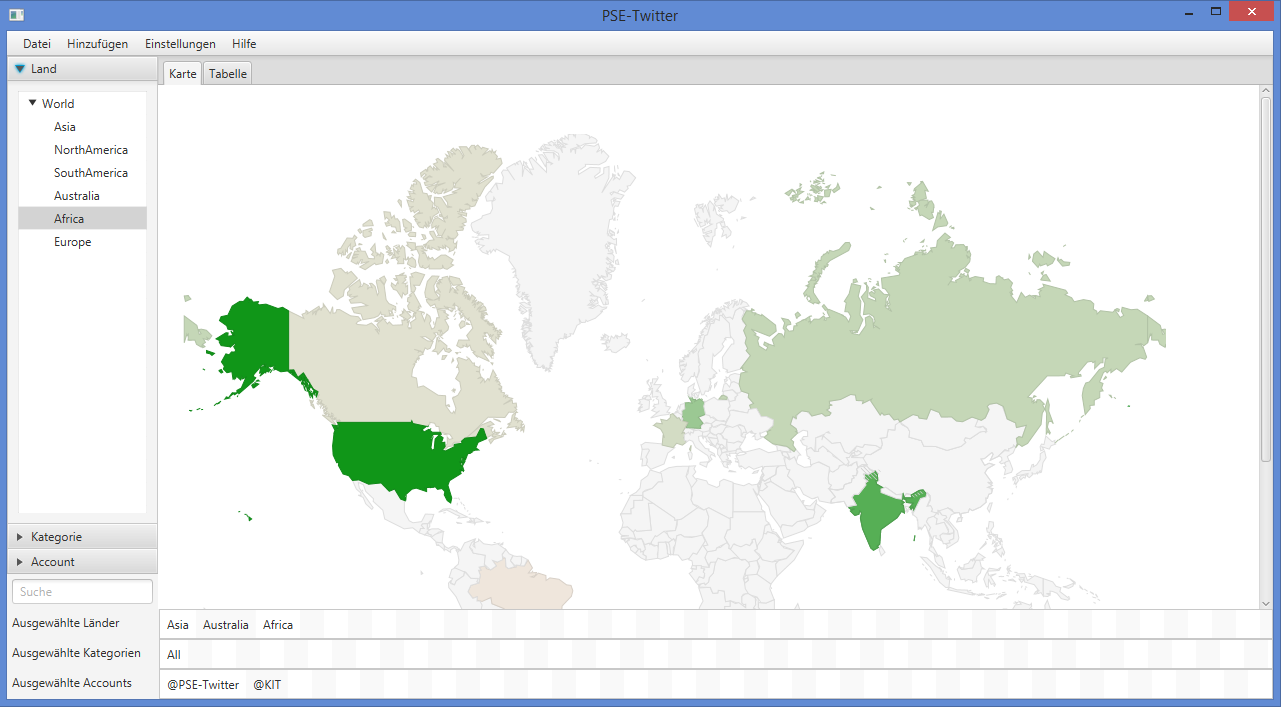
\includegraphics[width=0.9\textwidth]{img/DemoGUIMain.png}
	\caption{Hauptfenster}
	\label{c:Hauptfenster}
\end{figure}

\begin{description}
	\item[Landauswahl] In einer Baumstruktur werden Länder angezeigt. Die Auswahl einzelner Länder erfolgt durch Doppelklick auf das jeweilige Item.
	\item[Kategorienauswahl] Die Kategorien der DMOZ.org Datenbank werden als Baumstruktur angezeigt. Auswahl der Kategorien erfolgt durch Doppelklick auf das jeweilige Item.
	\item[Accountauswahl] In einer Liste werden Accounts (aus der eigenen Datenbank) angezeigt, die man ebenfalls per Doppelklick auswählen kann.
	\item[Suchfeld] In diesem Textfeld kann ein Begriff eingegeben werden. Je nach geöffnetem Fenster wird nach Land, Kategorie oder Account gesucht.
	\item[Länderübersicht] Eine Liste der bereits ausgewählten Länder.
	\item[Kategorienübersicht] Eine Liste der bereits ausgewählten Kategorien.
	\item[Accountübersicht] Eine Liste der bereits ausgewählten Accounts.
	\item[Karte] Die Weltkarte zeigt zu Beginn nur die Umrisse der Länder. Nach Auswahl von Ländern, Kategorien oder Accounts wird die Karte je nach Verteilung der Retweets zur Auswahl eingefärbt.	
\end{description}

\section{Tabellenansicht}

\begin{figure}[h]
	\centering
	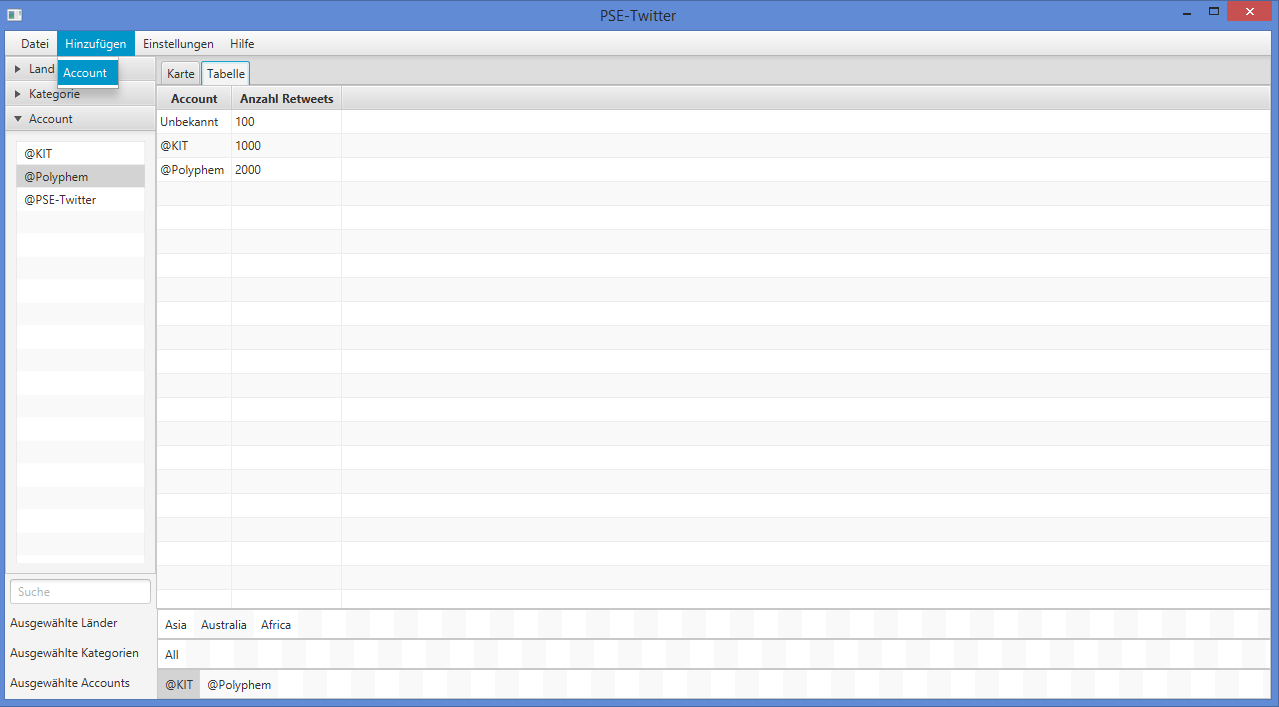
\includegraphics[width=0.9\textwidth]{img/DemoGUITabelleAddAccount.png}
	\caption{Tabellenansicht mit Menu}
	\label{c:Tabellenansicht mit Menu}
\end{figure}

\begin{description}
	\item[Hinzufügen-Menu] Menu-Eintrag, um einen weiteren (beliebigen) Twitter-Account hinzuzufügen. Klicken auf diesen Eintrag öffnet ein Fenster zum Hinzufügen eines Accounts.
	\item[Tabelle] Die Tabelle zeigt Informationen zu den einzelnen ausgewählten, zu Kategorien oder zu Ländern gehörenden Accounts.
\end{description}

\section{Fenster zum Hinzufügen von Accounts}

\begin{figure}[h]
	\centering
	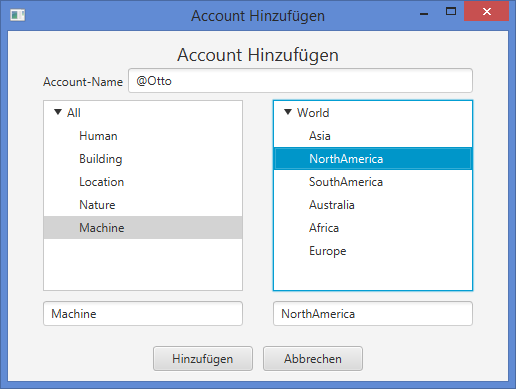
\includegraphics[width=0.9\textwidth]{img/DemoGUIAddAccount.png}
	\caption{Fenster zum Hinzufügen von Accounts}
	\label{c:Fenster zum Hinzufügen von Accounts}
\end{figure}

\begin{description}
	\item[Namensfeld] Textfeld zur Eingabe des Namens des hinzuzufügenden Accounts.
	\item[Hinzufügen-Button] Durch Drücken wird der eingegebene Account überprüft und gespeichert, sowie das Fenster geschlossen.
	\item[Abbrechen-Button] Dadurch wird der Hinzufügen-Vorgang unterbrochen und das Fenster geschlossen.
\end{description}

	\chapter{Qualitätszielbestimmungen}
		% Anforderungen  an  Stabilität,  Robustheit,  Leistungsfähigkeit  etc.  des Systems.  Dies  beinhaltet  auch  den  Umgang  mit  fehlerhaften  Eingabedaten  oder  fehlerhaften Konfigurationen.

	\chapter{Testfälle und Testszenarien}
		% Testfälle  für  die  einzelnen  Produktfunktionen,  die  alle  abgedeckt  sein müssen. Testszenarien für typische Anwendungsszenarien.

	\chapter{Entwicklungsumgebung}
		% Zur Entwicklung verwendete Hard‐ und Software. In der Pflichtenheft‐Phase soll  sich  das  Team  in  die  Werkzeuge  einarbeiten  und  sich  hier  vorläufig  festlegen.  Zu  diesen Werkzeugen zählen unter anderem ein UML‐Modellierungswerkzeug, IDE, Code‐Verwaltungssystem.

\section{Allgemein}
\begin{itemize}
	\item LaTeX
	\item Versionskontrolle (Git)
\end{itemize}
\section{Entwurf}
\begin{itemize}
	\item
\end{itemize}
\section{Implementierung}
\begin{itemize}
	\item Eclipse
	\item MySQL Workbench
\end{itemize}
\section{Validierung}
\begin{itemize}
	\item JUnit
	\item EclEmma
\end{itemize}
\section{Interne Kommunikation}
\begin{itemize}
	\item Email
\end{itemize}

	\chapter{Glossar}
		% Esentielle Begriffe.

\begin{description}

\end{description}

\end{document}
